The first version of the \gls{yolo} detection framework was published in 2015\cite{yolo}. It was, and still is, an hallmark in object detection; combining an \gls{map} comparable with other detection method at the time, but with a very impressive inference time. YOLO was one of the first detection method being able to infer in real time. YOLO is considered a "one stage" detector, meaning that the object localisation and classification is a part of the same method. It passes the image only one time through its \gls{cnn}, and directly outputs predictions; e.g it looks only once at the input. This dramatically increase the speed of the model. Since then, improvements\cite{yolov9000}\cite{yolov3} have been made to the model but the basic mechanism behind YOLO stays the same. For a review of the latest version, YOLOv4\cite{yolov4}, please refer to Section~\ref{yolov4}.  

In this section we will give a short explanation of the workings behind this framework.

\section{General Principle}
The main idea behind \gls{yolo} is to take the task of object classification and localisation as a regression task. The bounding boxes and class prediction are outputted directly as a tensor, without using a \gls{rpn}. This idea makes the network perform extremely fast.


YOLO can take as input image of various size, but it will first downscale them to a fixed resolution, which is a \gls{hyperparameter}. The input image is then divided into an $S \times S$ grid. Each grid cell predicts $B$ bounding boxes and confidence scores for these boxes. Each bounding box is comprised of 5 predictions : x, y, width, height and confidence. The $(x,y)$ are the position of the center of the bounding box relative to the grid cell. The confidence prediction represents the \gls{iou} between the predicted bounding box and the ground truth. Each grid cell also predict $C$ conditional class probabilities: $P(\text{Class}_i|\text{Object})$ , which are conditioned on the grid cell containing an object. 

$S, B$ and $C$ are also \gls{hyperparameter}, with $C$ being the number of classes. 

\begin{figure}[h!]
  \centering
  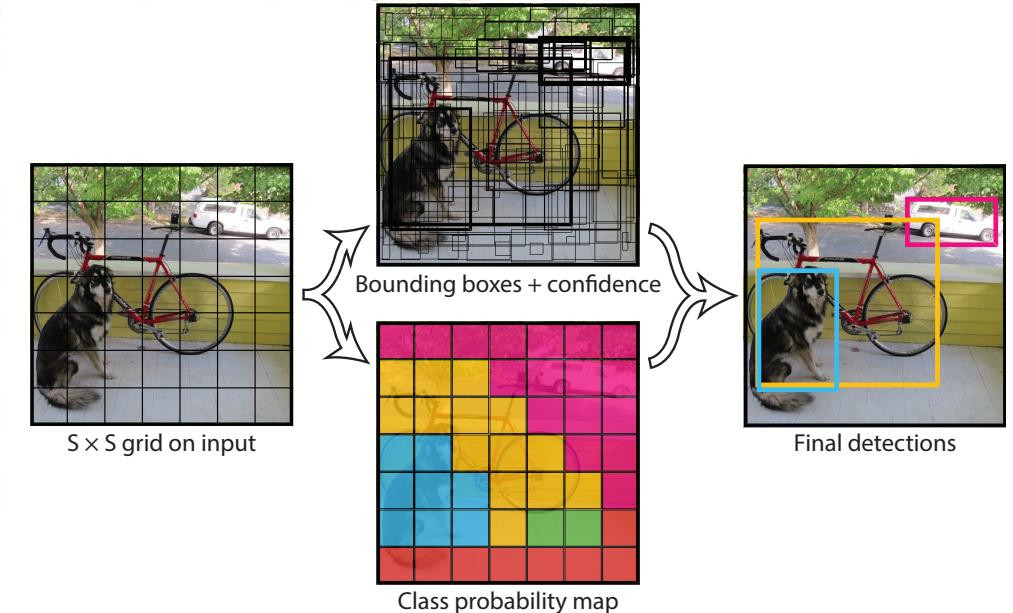
\includegraphics[width=\textwidth]{yoloGrid}
	\caption[YOLO model]{YOLO Model. First the image is divided into a $S \times S$, and for each grid cell predicts $B$ bounding boxes, confidence, and $C$ class scores, which are encoded into an $S \times S \times (B * 5 + C)$ tensor}
  \label{fig:yoloModel}
\end{figure}

\section{Network design and Architecture}
The backbone behind \gls{yolo} is called Darknet53 containing 53 layers. YOLOv3\cite{yolov3} introduced the idea of prediction at different scale. In the YOLOv3 network, 3 prediction are made at different scales, a technique known as multi-scale prediction which is improved in several papers of detection in satellite imagery, Multi-scale prediction allows the network to find small objects that are often missed otherwise. Figure~\ref{fig:yoloArchi} shows the architecture of the model.

\begin{figure}[h!]
  \centering
	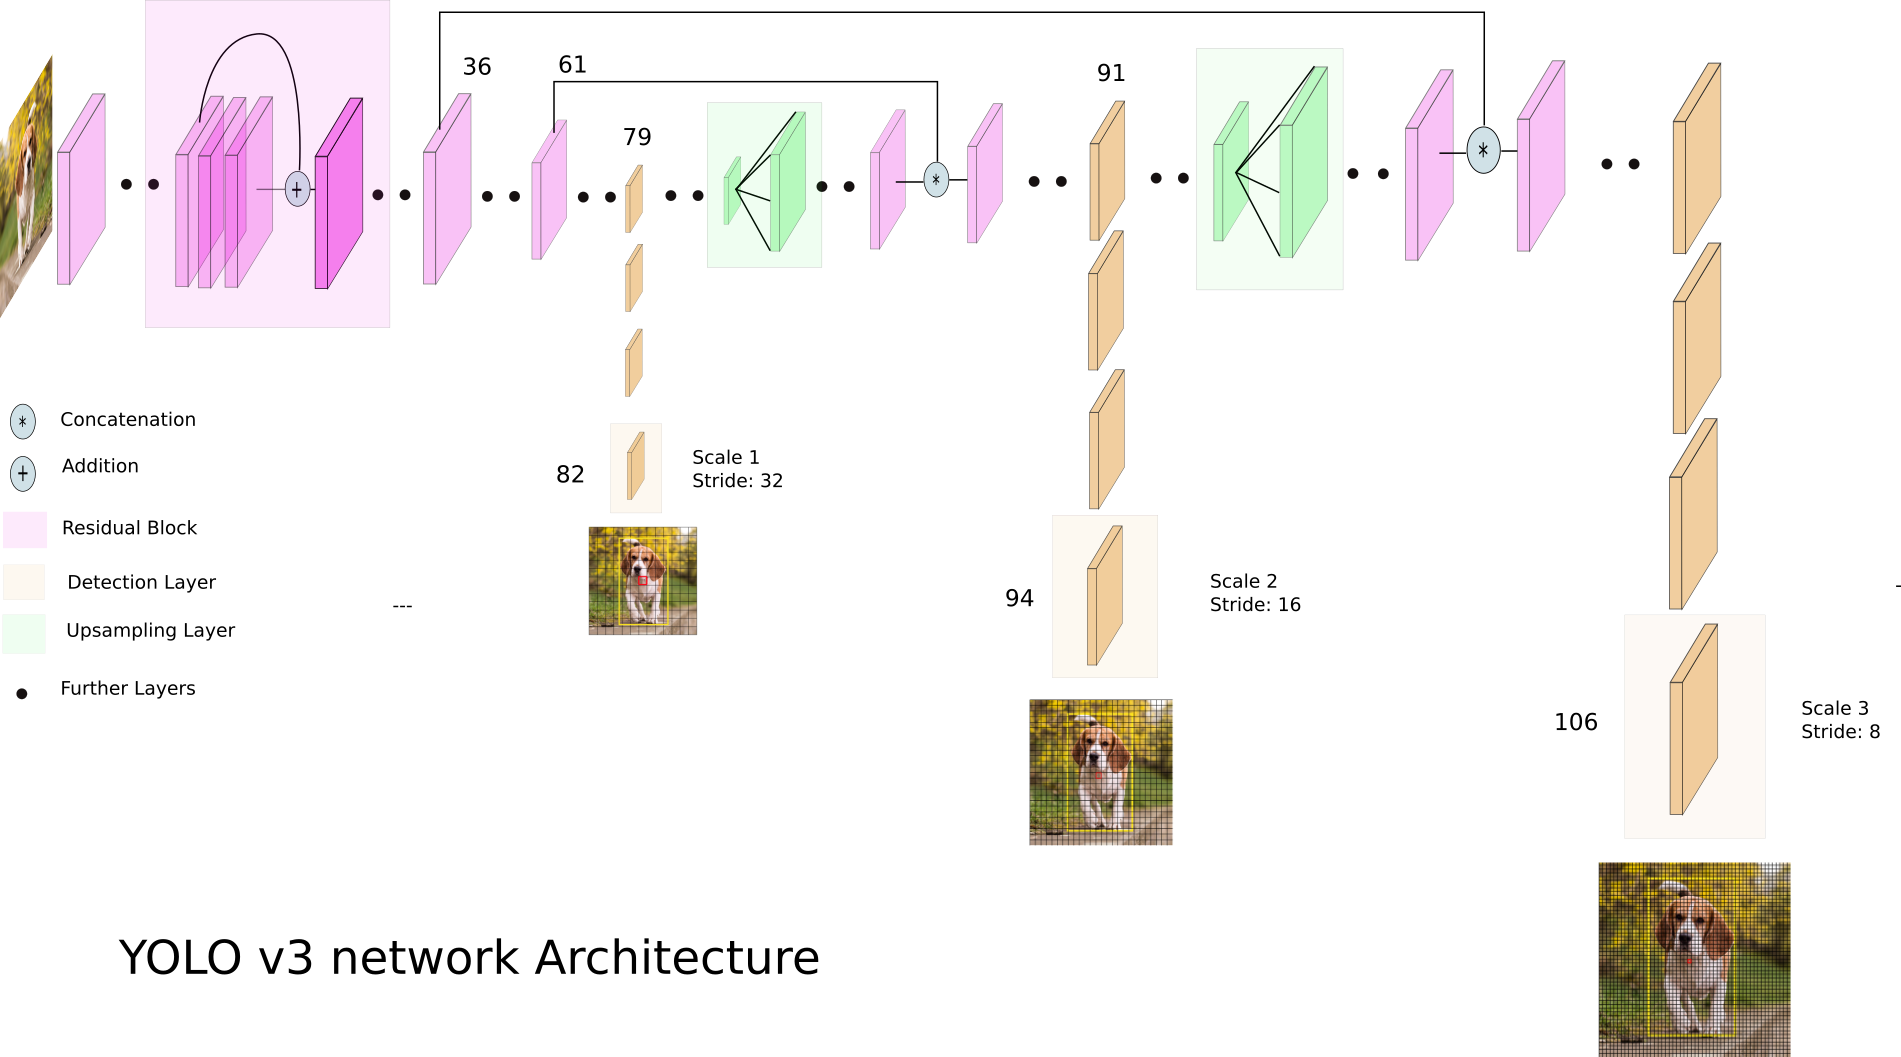
\includegraphics[width=\textwidth]{yoloArchi}
	\caption[Architecture of the backbone of the YOLO Framework]{Architecture of the backbone of the YOLO Framework}
  \label{fig:yoloArchi}
\end{figure}

